\chapter{光的量子化：从模式到光子}
\label{chap:e05}

\begin{chapteropening}
上一章我们把一个孤立的谐振子（harmonic oscillator）量子化了：能量只能一份一份地取，湮灭算符 \(\hat a\) 拿走一份能量，产生算符 \(\hat a^\dagger\) 添上一份。可那只是一个"弹簧"。真实望远镜面对的是充满整个空间、有颜色、有方向、有偏振、随时间起伏的电磁场。本章要做的，是把第 \ref{chap:e04} 章那一个谐振子的成功，成千上万倍地复制到整个光场上——办法只有一步：把光场先拆成一组"模式"（mode），然后惊讶地发现，每一个模式在数学上就是一个谐振子。于是"光子"这个词第一次获得精确定义：它不是一颗小球，而是某一个模式的一次激发。走完这一章，你会明白望远镜记录的每一次"点击"到底属于什么，也会算出一件反直觉的事：太阳那么亮，可每个光学模式里平均还不到百分之一个光子。
\end{chapteropening}

\section{为什么要把光场拆成"模式"}
\label{sec:e05-why-modes}

先问一个朴素的问题：电磁场是弥漫在整个空间的连续的东西，一个望远镜某一瞬间收到的是一大团振荡的场。我们要怎样把它"数成一份一份"？

答案的关键，是不要一上来就盯着"空间某点某时刻的场强"这种连续量，而是换一组更聪明的坐标。回忆第 \ref{chap:e02} 章的傅里叶分析（Fourier analysis）：任何一段复杂的声波，都可以唯一地写成一堆"纯音"（单一频率的正弦波）的叠加。纯音是声音世界里最简单、彼此独立的"积木"。**模式，就是电磁场版本的"广义纯音"。**

一个电磁场的模式，是一个同时被下面几件事标定的"积木"：

\begin{itemize}
  \item \textbf{频率}\(\ \omega\)（或颜色 \(\nu=\omega/2\pi\)）：这一块积木以多快的节奏振荡；
  \item \textbf{空间形状}\ \(u(\bm r)\)：这一块积木在空间里长什么样——是一束沿某方向传播的平面波，还是一个衍射受限的光斑，或是一根光纤里的导模；
  \item \textbf{偏振}（polarization）：电场矢量在垂直传播方向的平面里指向哪——水平、竖直，或某种旋转；
  \item \textbf{时间窗}\ \(\Delta t\)：这一块积木被"开着"的那段时间。
\end{itemize}

之所以要费劲选这样一组积木，是因为我们希望它们\emph{彼此正交、互不干扰}。正交（orthogonal）的意思和傅里叶里"不同频率的纯音相互独立"完全一样：把场沿这组模式展开，每个模式的系数可以单独测量、单独演化、单独量子化，不会互相牵扯。数学上，一组模式函数 \(\{u_k(\bm r)\}\) 满足正交归一
\[
  \int u_i^*(\bm r)\,u_j(\bm r)\,\mathrm d^3r=\delta_{ij},
\]
其中 \(\delta_{ij}\) 是克罗内克符号（Kronecker delta，\(i=j\) 时为 1，否则为 0）。有了这样一组"广义纯音"，麦克斯韦方程组允许我们把整个电磁场写成
\[
  \bm E(\bm r,t)=\sum_k\big[\,(\text{第 }k\text{ 个模式的振幅})\times u_k(\bm r)\,e^{-i\omega_k t}+\text{复共轭}\,\big].
\]
每一项都在以自己的频率 \(\omega_k\) 独立地振荡——这正是一个"广义纯音"应有的样子。下一节我们就盯住其中任意一个 \(k\)，看看它的振幅遵守什么运动方程。

\section{关键一步：每个模式就是一个谐振子}
\label{sec:e05-mode-is-oscillator}

现在把注意力锁定在单独一个模式 \(k\) 上。它的空间形状 \(u_k(\bm r)\) 是固定的，唯一还在动的，是它的振幅——记作 \(q_k(t)\)。我们要做的，是把这个单模式的场代进电磁场的能量密度、对空间积分，看它携带的总能量长什么样。这一步在标准电动力学里叫"场能量的模式展开"，很多教材（如 Jackson《经典电动力学》讲腔模的一节，或任意一本量子光学入门书的第一章）都会做；但它正是本章的\emph{地基}，跳过去自学读者就无法自证，所以我们把这段代数原原本本走一遍。真正要用到的只有三个事实，我们边走边点名。

\textbf{事实一：电磁场能量密度公式。}自由电磁场装在体积里的总能量是（CGS 单位）
\[
  U=\frac{1}{8\pi}\int\big(\bm E^2+\bm B^2\big)\,\mathrm d^3r,
\]
电场项和磁场项对称地各出一半——这是普通物理电磁学里就学过的结果，单位是 erg。

\textbf{事实二：单模式的场怎么写。}把式子里只保留第 \(k\) 个模式。取它是实驻波（腔模），电场可写成"空间形状 \(\times\) 随时间起伏的振幅"：
\[
  \bm E_k(\bm r,t)=-\,c_1\,\dot q_k(t)\,\bm u_k(\bm r),
\]
其中 \(\bm u_k\) 是上一节那个正交归一的模式函数、\(q_k(t)\) 是我们要盯住的振幅坐标，\(c_1\) 是一个只含常数（\(4\pi\)、\(c\) 等）的比例因子——先带着它，最后会被 \(q_k\) 的定义吸收掉。

\textbf{事实三：麦克斯韦方程把 \(\dot{\bm E}\) 和 \(\bm B\) 拴在一起。}真空里 \(\nabla\times\bm B=\tfrac1c\,\partial_t\bm E\)，所以磁场由电场的时间导数决定。把事实二的 \(\bm E_k\propto\dot q_k\,\bm u_k\) 代进去，右边 \(\propto\ddot q_k\,\bm u_k\)；对以 \(\omega_k\) 简谐振荡的模式 \(\ddot q_k=-\omega_k^2 q_k\)，于是磁场随时间的部分正比于 \(q_k(t)\) 本身，空间部分则由 \(\nabla\times\bm u_k\) 决定：
\[
  \bm B_k(\bm r,t)=c_2\,q_k(t)\,\big[\nabla\times\bm u_k(\bm r)\big].
\]
这里模式还满足亥姆霍兹方程 \(\nabla^2\bm u_k=-(\omega_k^2/c^2)\,\bm u_k\)——"空间形状的弯曲程度定出频率"——它待会儿会帮我们把磁场项的空间积分算成一个含 \(\omega_k^2\) 的数。

现在把事实二、三代进事实一的积分。电场项给出
\[
  \frac1{8\pi}\int\bm E_k^2\,\mathrm d^3r
  =\frac{c_1^2}{8\pi}\,\dot q_k^{\,2}\int|\bm u_k|^2\,\mathrm d^3r
  =\frac{c_1^2}{8\pi}\,\dot q_k^{\,2},
\]
最后一步正是用了上一节的\emph{正交归一} \(\int|\bm u_k|^2\,\mathrm d^3r=1\)，一下把空间积分做成了 1。同样地，磁场项里做同一个积分（用 \(\int|\nabla\times\bm u_k|^2\,\mathrm d^3r=(\omega_k^2/c^2)\int|\bm u_k|^2\,\mathrm d^3r=\omega_k^2/c^2\)，这一步用的就是亥姆霍兹方程）给出
\[
  \frac1{8\pi}\int\bm B_k^2\,\mathrm d^3r
  =\frac{c_2^2}{8\pi}\,q_k^{\,2}\cdot\frac{\omega_k^2}{c^2}
  \ \propto\ \omega_k^2\,q_k^{\,2}.
\]
于是电场项 \(\propto\dot q_k^{\,2}\)、磁场项 \(\propto\omega_k^2 q_k^{\,2}\)，两项一拼，能量就长成了"动能 + 势能"的谐振子模样：
\[
  U_k=(\text{常数}_1)\,\dot q_k^{\,2}+(\text{常数}_2)\,\omega_k^2\,q_k^{\,2}.
\]
最后一步是关键：那两个常数（都由 \(c_1,c_2,4\pi,c\) 等拼成）\emph{不是无关紧要的}。我们\textbf{把 \(q_k\) 重新定义}，让它把这些常数一并吸收进去（这在物理上总能做到：给振幅乘一个常数因子而已）。选好这个归一化，就是把 \(q_k\) 定义成这个模式的\emph{正则坐标}（canonical coordinate），等效质量取成 1。此时两项系数恰好都变成 \(\tfrac12\)，能量正好等于
\[
  H_k=\tfrac12\,\dot q_k^{\,2}+\tfrac12\,\omega_k^2\,q_k^{\,2}.
\]
把这行字读三遍。它和第 \ref{chap:e04} 章那个质量为 1 的弹簧的能量 \(H=\tfrac12\dot q^2+\tfrac12\omega^2 q^2\) \emph{一模一样}——注意这里是精确的\emph{等号}，而不是"正比于"：那个曾经含糊的比例常数，已经被我们对 \(q_k\) 的定义吃掉了，所以等效质量正好是 1 而不是别的系数。也就是说：

\begin{quote}
\textbf{每一个电磁场模式，在数学上就是一个频率为 \(\omega_k\) 的谐振子。}
\end{quote}

这是全章的枢纽。一旦承认这句话，我们就\emph{什么新东西都不用发明}——直接把第 \ref{chap:e04} 章对谐振子做过的量子化，逐字套到每个模式上。第 \ref{chap:e04} 章我们把 \(q,\dot q\) 打包成湮灭算符 \(\hat a\) 与产生算符 \(\hat a^\dagger\)。这里对第 \(k\) 个模式照做，得到一对 \(\hat a_k,\hat a_k^\dagger\)。因为不同模式彼此正交、互不干扰，它们的算符对易关系是

\begin{equation}
  [\hat a_i,\hat a_j^\dagger]=\delta_{ij},\qquad
  [\hat a_i,\hat a_j]=0,\qquad
  \hat n_k=\hat a_k^\dagger\hat a_k .
  \label{eq:e05-commutator}
\end{equation}
\begin{formulaexplain}
\(\hat a_k^\dagger,\hat a_k\) 在第 \(k\) 个模式里加一个、减一个光子；\(\delta_{ij}\) 说明只有\emph{同一个}模式的产生与湮灭才留下量子修正，不同模式完全独立；\(\hat n_k\) 数第 \(k\) 个模式里有几个光子。
\end{formulaexplain}

逐个交代记号。\(\hat a_k\) 是第 \(k\) 个模式的湮灭算符（annihilation operator），无量纲；它把该模式的激发数降一。\(\hat a_k^\dagger\) 是产生算符（creation operator），把激发数升一。对易子 \(\delta_{ij}\) 的物理含义是本章的重点之一：\(i\neq j\) 时 \([\hat a_i,\hat a_j^\dagger]=0\)，意味着"红光模式里的光子"和"蓝光模式里的光子"是两套毫不相干的账本，可以分别记数——这正是我们当初挑选\emph{正交}模式的回报。数算符 \(\hat n_k=\hat a_k^\dagger\hat a_k\) 的本征值是 \(N_k=0,1,2,\dots\)，是纯整数、没有单位，它数的就是"第 \(k\) 个模式里此刻有几份激发"。

一份激发，就是一个光子。到这里，"光子"终于有了不含糊的定义：光子不是空间里飞的一颗子弹，而是\emph{某一个确定模式（确定频率、确定空间形状、确定偏振）的能量升高了一整份}。同一个光子必然属于某个模式；问"这个光子在哪儿"，等价于问"它属于哪个模式"。

\section{正频率场算符：光子正式登场}
\label{sec:e05-field-operator}

把上一节每个模式的湮灭算符按空间形状和频率装配回去，就得到量子化之后的电场。物理上探测器真正"吸收光子"时用到的，是电场里只含 \(\hat a_k\)（湮灭）的那一半，称为\textbf{正频率场算符}（positive-frequency field operator）：

\begin{equation}
  \hat E^{(+)}(\bm r,t)=\sum_k \mathcal E_k\,u_k(\bm r)\,e^{-i\omega_k t}\,\hat a_k .
  \label{eq:e05-field-expansion}
\end{equation}
\begin{formulaexplain}
把光场写成一堆模式的和：第 \(k\) 项里，\(\mathcal E_k\) 是"一个光子有多强"的归一化系数，\(u_k(\bm r)\) 是模式的空间形状，\(e^{-i\omega_k t}\) 是它的振荡，\(\hat a_k\) 在这个模式里\emph{拿走一个光子}。整条式子就是"探测器看到的光"。
\end{formulaexplain}

逐个符号讲清楚，这条式子是后面所有章节的地基。

\begin{itemize}
  \item \(\hat E^{(+)}(\bm r,t)\)：正频率电场算符，含"湮灭"部分。\(\bm r\) 是位置（单位 cm），\(t\) 是时间（单位 s）。
  \item \(\mathcal E_k\)：单光子场强，即"这个模式里放一个光子对应多大的电场"的归一化因子。它把无量纲的算符 \(\hat a_k\) 换算成真正的场强（CGS 下单位 \(\mathrm{statvolt\,cm^{-1}}\)）。它由该模式的频率和有效体积定出，量级上 \(\mathcal E_k\propto\sqrt{\hbar\omega_k/V}\)——这里 \(V\) 是模式的有效体积（单位 cm\(^3\)），\(\hbar=h/2\pi\) 是约化普朗克常数（\(h\) 为普朗克常数，见第 \ref{sec:e05-occupation} 节），分子 \(\hbar\omega_k=h\nu_k\) 正是一个光子的能量。频率越高、模式体积越小，单个光子的场就越强。
  \item \(u_k(\bm r)\)：第 \(k\) 个模式的空间模式函数，无量纲（已按上一节正交归一），装载"这块积木长什么样、朝哪走"。
  \item \(e^{-i\omega_k t}\)：该模式的时间振荡，\(\omega_k=2\pi\nu_k\) 是角频率（单位 \(\mathrm{rad\,s^{-1}}\)）。负号约定使它成为"正频率"部分。
  \item \(\hat a_k\)：湮灭算符。它是这条式子里唯一的"量子"成分——正因为它，电场不再是一个数，而是一个能改变光子数的算符。
\end{itemize}

那另一半（只含产生算符 \(\hat a_k^\dagger\) 的部分）到哪去了？它就是式 \eqref{eq:e05-field-expansion} 的厄米共轭（Hermitian conjugate）：
\[
  \hat E^{(-)}(\bm r,t)=\big[\hat E^{(+)}(\bm r,t)\big]^\dagger
  =\sum_k \mathcal E_k^*\,u_k^*(\bm r)\,e^{+i\omega_k t}\,\hat a_k^\dagger .
\]
把两半加起来 \(\hat{\bm E}=\hat E^{(+)}+\hat E^{(-)}\)，才是可观测（厄米）的完整电场算符。为什么要把它们拆开？因为\textbf{光电探测本质上是吸收}：探测器里一个电子被光"打"出来，靠的是从光场里\emph{取走}一个光子，这个过程只用得上湮灭算符 \(\hat a_k\)，也就是只用得上 \(\hat E^{(+)}\)。于是我们得到一句贯穿全书的话：

\begin{quote}
\textbf{探测一个光子，就是在某个模式里把光子数减少一个}，数学上是 \(\hat E^{(+)}\)（含 \(\hat a_k\)）作用在光态上。
\end{quote}

望远镜从不直接读出 \(\hat a_k\) 或 \(\hat E\)——它读出的是时间戳、像素、能量通道、偏振通道，这些都是 \(\hat n_k\) 或若干 \(\hat n\) 的相关经过仪器响应后的产物。但概念上，每一次点击背后都站着一个 \(\hat a_k\)：某个模式，少了一个光子。

\section{光的数态：Fock 态}
\label{sec:e05-fock}

既然每个模式都是谐振子，谐振子的能量本征态自然升级成光场的能量本征态。第 \(k\) 个模式里恰有 \(N_k\) 个光子的态记作 \(|N_k\rangle\)，满足 \(\hat n_k|N_k\rangle=N_k|N_k\rangle\)。把所有模式的占据数一起指定，就得到整个光场的一个\textbf{数态}，又叫\textbf{Fock 态}（Fock state）：

\begin{equation}
  |\{N_k\}\rangle=|N_1,N_2,N_3,\dots\rangle,
  \qquad
  \hat n_k\,|\{N_k\}\rangle=N_k\,|\{N_k\}\rangle .
  \label{eq:e05-fock}
\end{equation}
\begin{formulaexplain}
Fock 态就是一张"点名册"：第 1 个模式里 \(N_1\) 个光子、第 2 个模式里 \(N_2\) 个……每个数都确定、没有涨落。它是"每个模式里到底有几个光子"这一问题的精确答案态。
\end{formulaexplain}

这里 \(N_k=0,1,2,\dots\) 是第 \(k\) 个模式的光子数，纯整数无单位。数态的物理含义非常干脆：它把\emph{每一个模式的光子数都钉死了}，没有任何涨落。例如 \(|0,0,\dots\rangle\)（所有模式都空）就是电磁真空；\(|0,1,0,\dots\rangle\) 是"只有第 2 个模式里有一个光子、其余全空"的单光子态。用产生算符可以搭出任意 Fock 态，就像第 \ref{chap:e04} 章用 \(\hat a^\dagger\) 一级一级往上爬能量阶梯：
\[
  |\{N_k\}\rangle=\prod_k\frac{(\hat a_k^\dagger)^{N_k}}{\sqrt{N_k!}}\,|0\rangle,
\]
其中 \(\sqrt{N_k!}\) 是归一化因子（来源与第 \ref{chap:e04} 章单模式完全相同，此处对每个模式各归一化一次）。Fock 态是理解一切光态的"坐标基"：后面要遇到的相干态、热态，都会写成 Fock 态的叠加或混合。而它给出的最重要教训是：光携带的信息藏在\emph{光子数}和\emph{光子数的关联}里，而不是一条连续波形里。

\section{一个通道里到底有多少个模式}
\label{sec:e05-mode-count}

这里有个天文观测最容易踩的坑：数据文件里"一个通道"（一个像素、一个时间 bin、一个滤光片）几乎\emph{从来不是}单单一个量子模式，而是许许多多模式的总和。要把物理算对，就得先会数：一个观测通道里塞了多少个独立模式？

思路是"相空间的可分辨格子相乘"。模式的三类标签——时间、空间、偏振——彼此独立，所以总模式数是三者各自的格子数相乘。我们逐项来数。

\paragraph{时间模式。}一个带宽为 \(\Delta\nu\) 的波包，它"记得住自己相位"的时间——相干时间（coherence time）——约为 \(\tau_c\simeq1/\Delta\nu\)（这正是第 \ref{chap:e02} 章傅里叶"时间越短、频谱越宽"的结论）。所以一段长为 \(\Delta t\) 的观测时间窗里，装得下大约
\[
  \frac{\Delta t}{\tau_c}
\]
个互相独立的时间模式——每过一个 \(\tau_c\)，场就"忘记"了之前的相位，等于换了一块新积木。

\paragraph{空间模式。}衍射（diffraction）决定一个空间模式占多大的"光展量"（\'etendue，面积 \(\times\) 立体角）。一束衍射受限的单模光，其面积与立体角之积约为 \(A\Omega\sim\lambda^2\)（这是衍射极限 \(\Delta\theta\sim\lambda/D\) 的另一种写法）。若望远镜与后端合起来接收的光展量是 \(A\Omega\)，那么装得下的空间模式数约为
\[
  \frac{A\Omega}{\lambda^2}.
\]
一个衍射受限的点源成像给出 \(A\Omega\sim\lambda^2\)，即单空间模式；而被大气抖动（seeing）糊开的像、或耦合进一根粗光纤、或落在一个大像素上，就会一次收进许多空间模式。

\paragraph{偏振模式。}电场在垂直传播方向上有两个独立偏振方向。若观测没有把偏振投影到单一通道，就再乘上偏振模式数 \(N_{\rm pol}\)（通常是 1 或 2）。

三项相乘，得到有效模式数：

\begin{equation}
  M\simeq
  \underbrace{\frac{\Delta t}{\tau_c}}_{\text{时间}}\,
  \underbrace{\frac{A\Omega}{\lambda^2}}_{\text{空间}}\,
  \underbrace{N_{\rm pol}}_{\text{偏振}},
  \qquad
  \tau_c\simeq\frac1{\Delta\nu}\simeq\frac{\lambda^2}{c\,\Delta\lambda}.
  \label{eq:e05-mode-number}
\end{equation}
\begin{formulaexplain}
有效模式数 = 时间格子数 \(\times\) 空间格子数 \(\times\) 偏振数。它告诉你，一个观测通道其实是 \(M\) 个量子模式的平均；\(M\) 越大，量子涨落被稀释得越狠。
\end{formulaexplain}

最后那个 \(\tau_c\simeq\lambda^2/(c\,\Delta\lambda)\) 是怎么来的？由 \(\nu=c/\lambda\) 微分，\(|\mathrm d\nu|=(c/\lambda^2)\,|\mathrm d\lambda|\)，即带宽换算 \(\Delta\nu\simeq c\,\Delta\lambda/\lambda^2\)（这与第 \ref{chap:e02} 章的记号一致）；再取倒数就得到 \(\tau_c\simeq\lambda^2/(c\,\Delta\lambda)\)。

代入真实数字感受一下。取可见光 \(\lambda=500\,\mathrm{nm}=5\times10^{-5}\,\mathrm{cm}\)、滤光片带宽 \(\Delta\lambda=1\,\mathrm{nm}=10^{-7}\,\mathrm{cm}\)、\(c=3\times10^{10}\,\mathrm{cm\,s^{-1}}\)：
\[
  \Delta\nu\simeq\frac{c\,\Delta\lambda}{\lambda^2}
  =\frac{(3\times10^{10})(10^{-7})}{(5\times10^{-5})^2}\,\mathrm{Hz}
  \simeq1.2\times10^{12}\,\mathrm{Hz},
  \qquad
  \tau_c\simeq\frac1{\Delta\nu}\simeq0.8\,\mathrm{ps}.
\]
相干时间只有不到 1 皮秒（picosecond）！可是最快的光电探测器时间响应也在 \(100\,\mathrm{ps}\sim1\,\mathrm{ns}\) 量级。这意味着，即便探测器"跑得飞快"，一个时间 bin 里也已经压进了 \(\Delta t/\tau_c\sim10^2\)–\(10^3\) 个独立时间模式。再算上被 seeing 糊开的空间模式，一个天文通道动辄是\emph{成千上万个模式}的和。记住这句话，它会在后面解释为什么天体光的聚束、非经典信号总是被"稀释"得很浅：

\begin{quote}
\textbf{天文里的"一个通道"，通常不是一个量子模式，而是许多模式的总和。}
\end{quote}

\section{单模玻色占有数：每个模式其实很暗}
\label{sec:e05-occupation}

最后一个数量级，会彻底改变你对"恒星有多亮"的直觉。问题是：一颗恒星的连续谱光，平均\emph{每个模式里有几个光子}？

把某一个频率为 \(\nu\) 的模式当成一个和亮温为 \(T_b\) 的热库达到平衡的谐振子。这个模式里有 \(N\) 个光子时能量是 \(N h\nu\)（第 \ref{chap:e04} 章的能量阶梯，此处取零点能之上的部分）。热平衡下出现 \(N\) 个光子的概率由玻尔兹曼权重给出，正比于 \(e^{-Nh\nu/k_{\rm B}T_b}\)。为书写方便，记
\[
  x\equiv e^{-h\nu/k_{\rm B}T_b}\quad(0<x<1),\qquad
  P(N)=\frac{x^N}{\sum_{M=0}^{\infty}x^M}.
\]
分母是一个几何级数（geometric series），用公比为 \(x\) 的求和公式 \(\sum_{M=0}^{\infty}x^M=1/(1-x)\)（因 \(0<x<1\) 收敛），于是归一化后的概率是几何分布
\[
  P(N)=(1-x)\,x^N .
\]
现在求平均占有数 \(\bar n_\nu=\langle N\rangle=\sum_{N=0}^{\infty}N\,P(N)\)。关键是那一步含 \(N\) 的求和。用一个标准技巧：对几何级数逐项求导，
\[
  \sum_{N=0}^{\infty}N\,x^N
  =x\,\frac{\mathrm d}{\mathrm dx}\sum_{N=0}^{\infty}x^N
  =x\,\frac{\mathrm d}{\mathrm dx}\!\left(\frac1{1-x}\right)
  =\frac{x}{(1-x)^2}.
\]
代回去，那个 \((1-x)\) 恰好约掉一次：
\[
  \bar n_\nu=(1-x)\sum_{N=0}^{\infty}N\,x^N
  =(1-x)\cdot\frac{x}{(1-x)^2}
  =\frac{x}{1-x}
  =\frac1{\,1/x-1\,}.
\]
把 \(1/x=e^{+h\nu/k_{\rm B}T_b}\) 代回，就得到本章的收官公式——单模玻色占有数（single-mode boson occupation），即普朗克分布里那个熟悉的因子：

\begin{equation}
  \bar n_\nu=\frac1{\exp(h\nu/k_{\rm B}T_b)-1}.
  \label{eq:e05-occupation}
\end{equation}
\begin{formulaexplain}
\(\bar n_\nu\) 是"平均每个模式里有几个光子"。\(h\nu\) 是一个光子的能量，\(k_{\rm B}T_b\) 是亮温对应的热能；两者之比大，占有数就指数地小。它衡量的是"每模式光子多不多"，而不是"总光子多不多"。
\end{formulaexplain}

逐项交代单位。\(h\nu\) 与 \(k_{\rm B}T_b\) 都是能量（CGS 下单位 erg）：\(h\) 是普朗克常数，\(k_{\rm B}\) 是玻尔兹曼常数，\(T_b\) 是亮温（单位 K）。\(\bar n_\nu\) 无量纲，就是一个纯粹的"平均光子数"。

代入太阳。取恒星表面亮温 \(T_b=5800\,\mathrm{K}\)、波长 \(\lambda=500\,\mathrm{nm}\)。光子能量 \(h\nu=hc/\lambda\)。用便捷单位 \(hc\simeq1240\,\mathrm{eV\,nm}\)，得 \(h\nu\simeq1240/500\simeq2.48\,\mathrm{eV}\)；热能 \(k_{\rm B}T_b\simeq(8.62\times10^{-5}\,\mathrm{eV\,K^{-1}})(5800\,\mathrm{K})\simeq0.50\,\mathrm{eV}\)。于是那个决定一切的比值是
\[
  \frac{h\nu}{k_{\rm B}T_b}\simeq\frac{2.48}{0.50}\simeq5.0 .
\]
代进式 \eqref{eq:e05-occupation}：
\[
  \bar n_\nu\simeq\frac1{e^{5}-1}=\frac1{148.4-1}\simeq6.8\times10^{-3}
  \approx7\times10^{-3}.
\]
每个光学模式里平均只有大约\emph{百分之零点七个光子}。换句话说，绝大多数模式在绝大多数相干时间窗里是\emph{空的}，只有偶尔某个模式里蹦出一个光子。这就是可见光天文所处的"每模式弱光极限"（few-photon-per-mode regime）。

这里一定要把两件事分清楚，否则会被"太阳好亮"的直觉带偏：

\begin{quote}
\textbf{总光子率高，绝不等于每个模式里光子多。}
\end{quote}

太阳每秒往望远镜里灌进海量光子，是因为它同时点亮了\emph{天文数字般多}的模式（\(M\) 极大，见上一节），而不是因为每个模式很"满"。每个模式本身其实很暗，\(\bar n_\nu\sim10^{-2}\)。这个数量级会随波长变化：到近红外 \(\lambda=1\,\mu\mathrm{m}\) 时 \(h\nu/k_{\rm B}T_b\) 减半，\(\bar n_\nu\) 升到约 \(0.09\)；到中红外 \(10\,\mu\mathrm{m}\) 可超过 1；而射电、毫米波因为 \(h\nu\ll k_{\rm B}T_b\)，进入 \(\bar n_\nu\gg1\) 的强占有数、近经典波动区（Rayleigh--Jeans 区）。天体里的天体脉泽（astrophysical maser，如水脉泽、羟基脉泽）更是极端例子：它们在射电/毫米波波段的亮温可高达 \(10^{12}\)\,K 以上，单模占有数 \(\bar n_\nu\) 因而巨大，光子挤在同一个模式里，行为几乎纯粹是经典波。图 \ref{fig:e05-mode-occupation} 把这条随波长和亮温变化的曲线画了出来（图中只画了三条普通黑体曲线，脉泽的亮温远在图外）。

\begin{figure}[tbp]
\centering
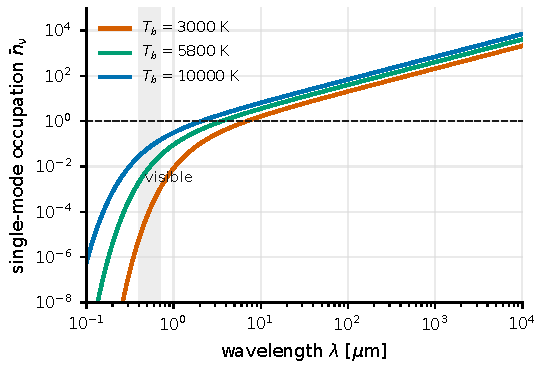
\includegraphics[width=0.82\linewidth]{figures/generated/chapter_03/ch03_blackbody_mode_occupation.pdf}
\caption{三条不同亮温黑体（3000、5800、10000\,K）的单模占有数 \(\bar n_\nu\) 随波长的变化，灰带标出可见光波段，虚线标出 \(\bar n_\nu=1\)。可见光灰带内，即便亮温是太阳量级，\(\bar n_\nu\) 也远小于 1（\(\sim10^{-2}\)），说明光学恒星光处在每模式弱光极限；向长波（红外、毫米波）一端，各温度曲线依次越过 \(\bar n_\nu=1\) 的虚线，进入 \(h\nu\ll k_{\rm B}T_b\) 的强占有数、近经典（Rayleigh--Jeans）极限。}
\label{fig:e05-mode-occupation}
\end{figure}

为什么这个"每模式很暗"如此要紧？因为它正是后面几章的出发点。既然每个相干时间窗里通常没有光子、偶尔才有一个，那么携带天体空间信息的，往往就是那一个被探测到的光子所在的模式——这直接引出弱热光（weak thermal light）的统计、光子成对到达的关联，以及超越衍射极限的量子超分辨（quantum super-resolution）思想。带着"太阳的每个模式其实很暗"这句话，我们就能进入下一阶段：看这些稀疏的光子在探测器上留下怎样的统计指纹。

\section{本章要点}
\label{sec:e05-summary}

\begin{itemize}
  \item \textbf{模式是光场的"广义纯音"。}把电磁场按一组正交模式（频率、空间形状、偏振、时间窗）展开，是傅里叶思想在电磁场上的推广，好处是每个模式彼此独立、可分别量子化。
  \item \textbf{每个模式就是一个谐振子。}这是全章枢纽：于是第 \ref{chap:e04} 章的量子化原样套上，得到每模式的 \(\hat a_k,\hat a_k^\dagger\)、对易关系 \([\hat a_i,\hat a_j^\dagger]=\delta_{ij}\) 和数算符 \(\hat n_k=\hat a_k^\dagger\hat a_k\)。
  \item \textbf{光子 = 某个模式的一次激发。}正频率场算符 \(\hat E^{(+)}=\sum_k\mathcal E_k u_k(\bm r)e^{-i\omega_k t}\hat a_k\) 里唯一的量子成分是 \(\hat a_k\)；探测一个光子就是在某模式里减少一个光子。\(\hat E^{(-)}\) 是它的厄米共轭。
  \item \textbf{Fock 态 \(|\{N_k\}\rangle\)} 把每个模式的光子数都钉死，是理解一切光态的坐标基。
  \item \textbf{一个观测通道往往是许多模式的和}：\(M\simeq(\Delta t/\tau_c)(A\Omega/\lambda^2)N_{\rm pol}\)，可见光下轻易达到成千上万。
  \item \textbf{光学恒星光处在每模式弱光极限}：\(\bar n_\nu=[\exp(h\nu/k_{\rm B}T_b)-1]^{-1}\)，太阳量级下 \(\bar n_\nu\approx7\times10^{-3}\)。总光子率高 \(\neq\) 每模式光子多。
\end{itemize}

\medskip
\noindent\textbf{想一想。}
\begin{enumerate}
  \item 若把滤光片带宽 \(\Delta\lambda\) 放宽 10 倍，相干时间 \(\tau_c\) 和一个 \(\Delta t\) 时间窗里的时间模式数各怎么变？
  \item 一根接收 seeing 糊开像的粗光纤，和一台衍射受限的成像仪，哪个的空间模式数 \(A\Omega/\lambda^2\) 更大？这对"看到的量子涨落深浅"意味着什么？
  \item 对同一颗恒星，为什么在 \(10\,\mu\mathrm{m}\) 中红外观测时，"每模式弱光"的图像会失效？用式 \eqref{eq:e05-occupation} 估一估此时的 \(\bar n_\nu\)。
\end{enumerate}
